\documentclass[10pt]{beamer}
\usepackage{tikz}
\usetikzlibrary{positioning}
\usepackage{pgfplots}
\usepackage{booktabs}
\usepackage{multirow}
\usepackage{array}
\usepackage{siunitx}
\usepackage{makecell}
\usepackage{CJKutf8}
\usepackage{hyperref}
\usepackage{tikz}

\pgfplotsset{compat=newest}
\setbeamertemplate{navigation symbols}{}

% Add page number to the lower right corner
\setbeamertemplate{footline}{%
  \hfill\usebeamercolor[fg]{page number in head/foot}%
  \usebeamerfont{page number in head/foot}%
  \insertframenumber\,/\,\inserttotalframenumber\hspace*{1ex}\vskip2pt%
}
\setbeamercolor{page number in head/foot}{fg=gray}
\setbeamerfont{page number in head/foot}{size=\small}

\title{Git \& GitHub}
\author{Tzu-You Lin}
\setbeamerfont{title}{size=\huge}
\date{May 21, 2025}

\begin{document}

\begin{frame}
    \titlepage
\end{frame}

\begin{frame}
    \frametitle{Outline}
    \begin{itemize}
        \item Introduction to Version Control and Git
        \item Git Workflow and Stages
        \item Basic Git Commands: Status, Add, Commit
        \item Viewing History and Differences
        \item Branching, Merging, and Conflict Resolution
        \item Working with Remote Repositories and GitHub
        \item Collaboration, Workflows, and Best Practices
        \item Advanced Topics and Further Resources
    \end{itemize}
\end{frame}

\begin{frame}
    \frametitle{What is Version Control?}
    \begin{itemize}
        \item A system to track changes in files over time.
        \item Enables reverting to previous states and efficient collaboration.
        \item Essential for software development and team projects.
    \end{itemize}
\end{frame}

\begin{frame}
    \frametitle{What is Git?}
    \begin{itemize}
        \item A distributed version control system developed by Linus Torvalds in 2005.
        \item Provides fast performance, robust branching, and decentralized workflows.
        \item Every developer's working copy is a full-fledged repository.
    \end{itemize}
\end{frame}

\begin{frame}
    \frametitle{Why Use Git?}
    \begin{itemize}
        \item Fast local operations and history tracking.
        \item Powerful branching and merging capabilities.
        \item Enables smooth collaboration across distributed teams.
        \item Backed by a vast community and extensive documentation.
    \end{itemize}
\end{frame}

\begin{frame}
    \frametitle{Installing Git}
    \begin{itemize}
        \item \textbf{Windows:} Download from \url{https://git-scm.com/download/win}.
        \item \textbf{macOS:} Use Homebrew (\texttt{brew install git}) or download from \url{https://git-scm.com/download/mac}.
        \item \textbf{Linux:} Install via package manager, e.g., \texttt{sudo apt-get install git} on Debian/Ubuntu.
    \end{itemize}
\end{frame}

\begin{frame}
    \frametitle{Understanding Git: The Game Analogy}
    \begin{itemize}
        \item \textbf{Starting a New Game:} \texttt{git init} creates a new game world.
        \item \textbf{Save Points:} Each \texttt{commit} is like saving your game progress.
        \item \textbf{Multiple Save Files:} \texttt{branches} are like different game paths.
        \item \textbf{Loading a Save:} \texttt{git checkout} lets you go back to any previous save point.
    \end{itemize}

    \vspace{0.5em}
    \centering
    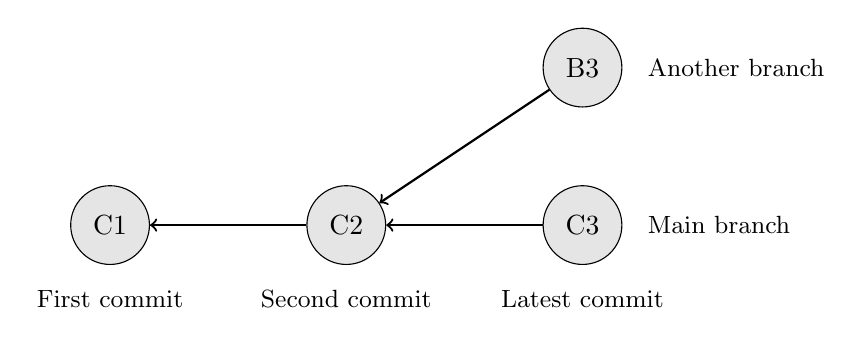
\begin{tikzpicture}[
        commit/.style={circle, draw, fill=gray!20, minimum size=1cm},
        arrow/.style={->, thick}
    ]
        \node[commit] (c1) at (0,0) {C1};
        \node[commit] (c2) at (3,0) {C2};
        \node[commit] (c3) at (6,0) {C3};
        \node[commit] (b3) at (6,2) {B3};
        
        \draw[arrow] (c2) -- (c1);
        \draw[arrow] (c3) -- (c2);
        \draw[arrow] (b3) -- (c2);
        
        \node[below=0.2cm of c1] {\small First commit};
        \node[below=0.2cm of c2] {\small Second commit};
        \node[below=0.2cm of c3] {\small Latest commit};
        \node[right=0.2cm of b3] {\small Another branch};
        \node[right=0.2cm of c3] {\small Main branch};
    \end{tikzpicture}
\end{frame}

\begin{frame}
    \frametitle{Initializing a Repository}
    \begin{itemize}
        \item \texttt{git init} creates a new local repository.
        \item \texttt{git clone [url]} copies an existing repository.
        \item A hidden \texttt{.git} folder stores all versioning data.
    \end{itemize}
\end{frame}

\begin{frame}
    \frametitle{Understanding Git Stages}
    \begin{itemize}
        \item \textbf{Working Directory:} Your local files where you make changes.
        \item \textbf{Staging Area (Index):} A temporary area where changes are prepared before committing.
        \item \textbf{Repository:} The history of all commits.
    \end{itemize}
    \vspace{0.5em}
    \centering
    \emph{Workflow:} Edit in the working directory $\rightarrow$ Stage changes $\rightarrow$ Commit to the repository.

    \vspace{0.5em}
    \begin{figure}
        \centering
        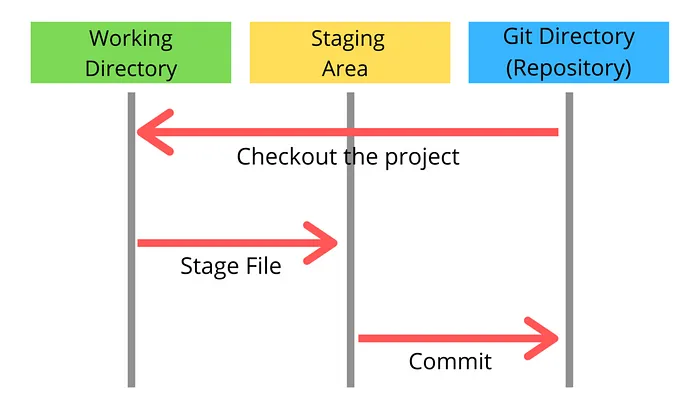
\includegraphics[width=0.7\textwidth]{stages.jpg}
    \end{figure}
\end{frame}

\begin{frame}
    \frametitle{Git Status}
    \begin{itemize}
        \item Use \texttt{git status} to check the current state.
        \item Displays which files are modified, staged, or untracked.
        \item Helps you understand what changes need to be staged or committed.
    \end{itemize}
\end{frame}

\begin{frame}
    \frametitle{Git Add}
    \begin{itemize}
        \item Use \texttt{git add [file]} to move changes from the working directory to the staging area.
        \item Prepares specific changes for the next commit.
        \item You can add individual files or use \texttt{git add .} to stage all changes.
    \end{itemize}
\end{frame}

\begin{frame}
    \frametitle{Git Commit}
    \begin{itemize}
        \item Use \texttt{git commit -m "message"} to record the staged changes.
        \item Each commit represents a snapshot of your project at a given time.
        \item Write clear commit messages to document your changes.
    \end{itemize}
\end{frame}

\begin{frame}
    \frametitle{Viewing History \& Changes}
    \begin{itemize}
        \item \texttt{git log} displays the commit history.
        \item \texttt{git diff} shows the changes between commits or between the working directory and the staging area.
        \item \texttt{git blame [file]} helps identify who modified specific lines.
    \end{itemize}
\end{frame}

\begin{frame}
    \frametitle{Why Branch and Merge?}
    \begin{itemize}
        \item \textbf{Branching Benefits:}
        \begin{itemize}
            \item Isolate new feature development from stable code
            \item Work on multiple features simultaneously
            \item Experiment without affecting the main codebase
            \item Quick fixes without disrupting ongoing work
        \end{itemize}
        \vspace{0.3em}
        \item \textbf{Common Branch Types:}
        \begin{itemize}
            \item \texttt{main/master} - Primary production branch
            \item \texttt{feature/*} - New features development
            \item \texttt{hotfix/*} - Urgent production fixes
        \end{itemize}
    \end{itemize}

    \vspace{0.3em}
    \centering
    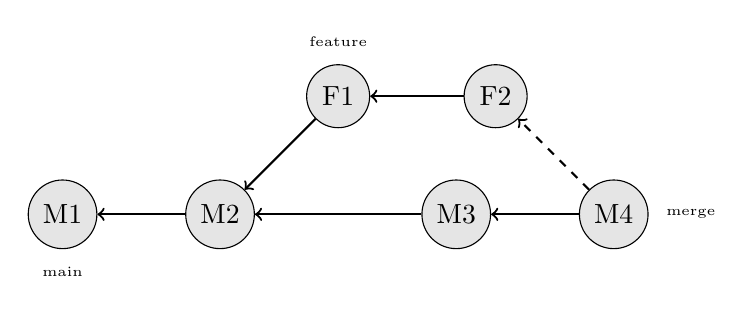
\begin{tikzpicture}[
        commit/.style={circle, draw, fill=gray!20, minimum size=0.8cm},
        arrow/.style={->, thick}
    ]
        \node[commit] (m1) at (0,0) {M1};
        \node[commit] (m2) at (2,0) {M2};
        \node[commit] (m3) at (5,0) {M3};
        \node[commit] (m4) at (7,0) {M4};
        \node[commit] (f1) at (3.5,1.5) {F1};
        \node[commit] (f2) at (5.5,1.5) {F2};
        
        \draw[arrow] (m2) -- (m1);
        \draw[arrow] (m3) -- (m2);
        \draw[arrow] (m4) -- (m3);
        \draw[arrow] (f1) -- (m2);
        \draw[arrow] (f2) -- (f1);
        \draw[arrow, dashed] (m4) -- (f2);
        
        \node[below=0.1cm of m1] {\tiny main};
        \node[above=0.1cm of f1] {\tiny feature};
        \node[right=0.1cm of m4] {\tiny merge};
    \end{tikzpicture}
\end{frame}

\begin{frame}
    \frametitle{Branch and Merge Commands}
    \begin{itemize}
        \item \textbf{Common Branch Commands:}
        \begin{itemize}
            \item \texttt{git branch} - List all branches
            \item \texttt{git branch [name]} - Create new branch
            \item \texttt{git checkout -b [name]} - Create and switch to new branch
            \item \texttt{git branch -d [name]} - Delete a branch
        \end{itemize}
        \vspace{0.3em}
        \item \textbf{Merging Commands:}
        \begin{itemize}
            \item \texttt{git merge [branch]} - Merge specified branch into current branch
            \item \texttt{git merge --abort} - Cancel merge if conflicts occur
            \item \texttt{git merge --no-ff} - Create merge commit even if fast-forward possible
        \end{itemize}
    \end{itemize}
\end{frame}

\begin{frame}[fragile]
    \frametitle{Resolving Merge Conflicts}
    \begin{itemize}
        \item Conflicts look like this in your files:
        \begin{verbatim}
<<<<<<< HEAD
Your current changes
=======
Changes from other branch
>>>>>>> feature
        \end{verbatim}
        \item Steps to resolve:
        \begin{enumerate}
            \item Run \texttt{git status} to see conflicted files
            \item Open each file and choose which changes to keep
            \item Remove conflict markers (\texttt{<<<<<<<}, \texttt{=======}, \texttt{>>>>>>>})
            \item \texttt{git add} the resolved files
            \item \texttt{git commit} to complete the merge
        \end{enumerate}
        \item Use \texttt{git merge --abort} to start over if needed
    \end{itemize}
\end{frame}

\begin{frame}
    \frametitle{Introduction to GitHub}
    \begin{itemize}
        \item A web-based platform for hosting Git repositories.
        \item \textbf{Why use GitHub?}
        \begin{itemize}
            \item Backup and access code from anywhere
            \item Easy collaboration with other developers
            \item Track issues and manage projects
            \item Showcase your work to potential employers
        \end{itemize}
        \item Provides collaboration features such as pull requests, issues, and wikis.
        \item Integrates with continuous integration and deployment tools.
    \end{itemize}
\end{frame}

\begin{frame}
    \frametitle{Understanding Remote Operations}
    \begin{itemize}
        \item \textbf{Remote Repository:}
        \begin{itemize}
            \item A version of your project hosted on the internet/network
            \item Acts as the central source of truth for collaboration
            \item Contains all branches and history
        \end{itemize}
        \vspace{0.3em}
        \item \textbf{Remote Operations:}
        \begin{itemize}
            \item \texttt{fetch}: Downloads commits/refs from remote but doesn't integrate them
            \item \texttt{pull}: Combines \texttt{fetch} + \texttt{merge} to update local branch
            \item \texttt{pull --rebase}: Combines \texttt{fetch} + \texttt{rebase} for cleaner history
            \item \texttt{push}: Uploads local commits to remote repository
        \end{itemize}
        \vspace{0.3em}
        \item \textbf{Tracking Branches:}
        \begin{itemize}
            \item Local branches that map to remote branches (e.g., \texttt{origin/main})
            \item Enable easy synchronization between local and remote
        \end{itemize}
    \end{itemize}
\end{frame}

\begin{frame}
    \frametitle{Remote Repository States}
    \begin{figure}
        \centering
        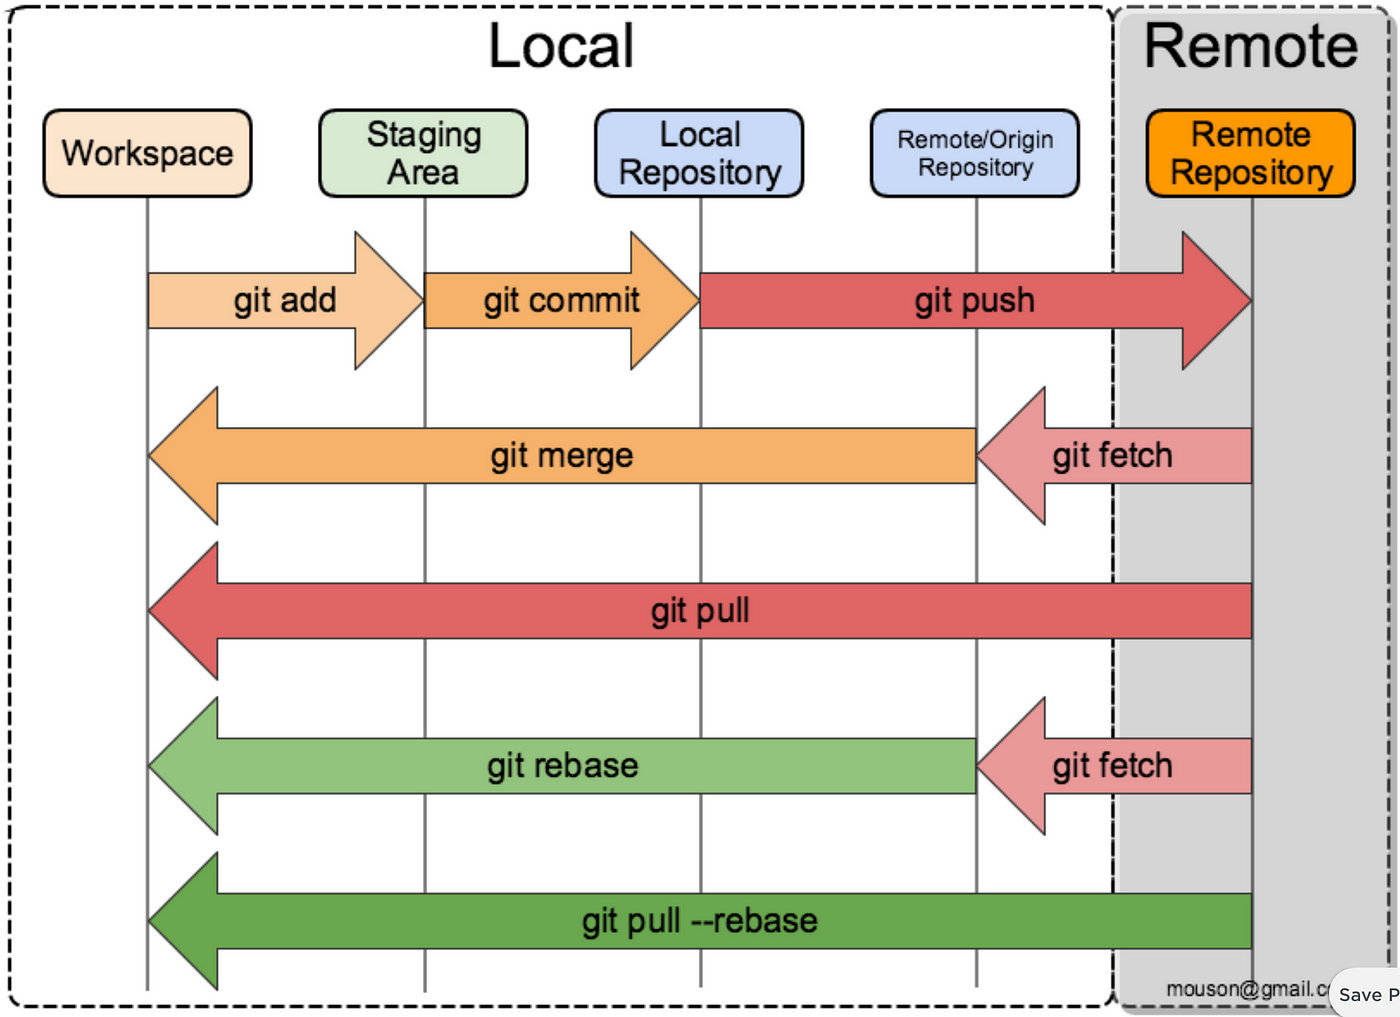
\includegraphics[width=0.9\textwidth]{stage_remote.png}
    \end{figure}
\end{frame}

\begin{frame}
    \frametitle{Working with Remote Repositories}
    \begin{itemize}
        \item \texttt{git remote add [name] [url]} connects your local repo to a remote repository.
        \item \texttt{git fetch} retrieves updates from the remote.
        \item \texttt{git pull} combines fetch and merge to update your local branch.
        \item \texttt{git push} uploads local commits to the remote repository.
    \end{itemize}
\end{frame}

\begin{frame}
    \frametitle{Creating a GitHub Repository}
    \begin{itemize}
        \item Sign up at \url{https://github.com} and log in.
        \item Click \texttt{New Repository} and fill in the repository details.
        \item Choose Public or Private; optionally initialize with a README.
        \item Clone the repository locally with \texttt{git clone}.
    \end{itemize}
\end{frame}

\begin{frame}
    \frametitle{Collaborating on GitHub}
    \begin{itemize}
        \item \textbf{Forking:} Create a personal copy of someone else's repository.
        \item \textbf{Pull Requests:} Propose changes to the original repository.
        \item Engage in code reviews, discussions, and issue tracking.
    \end{itemize}
\end{frame}

\begin{frame}
    \frametitle{Advanced Commands \& Best Practices}
    \begin{itemize}
        \item \texttt{git stash} - Temporarily save uncommitted changes.
        \item \texttt{git rebase} - Reapply commits on top of another base.
        \item \texttt{git cherry-pick} - Apply specific commits to your current branch.
        \item Write clear commit messages, commit small changes, and pull updates regularly.
    \end{itemize}
\end{frame}

\begin{frame}
    \frametitle{Resources \& Further Learning}
    \begin{itemize}
        \item \textbf{Official Git Documentation:} \url{https://git-scm.com/doc}
        \item \textbf{GitHub Guides:} \url{https://guides.github.com}
        \item \textcolor{blue}{\textbf{Interactive Tutorial:} \url{https://learngitbranching.js.org/}}
        \item \textbf{Onnline Resources:} There are a lot of lecture videos on YouTube.
    \end{itemize}
\end{frame}

\end{document}
